\documentclass[10pt,a4paper]{article}

\usepackage[a4paper,left=16mm,right=16mm,top=15mm,bottom=13mm]{geometry}
\usepackage{fontspec}
\usepackage{xcolor}
\usepackage{graphicx}
\usepackage{tikz}
\usepackage{tabularx}
\usepackage{parskip}
\usepackage{microtype}
\usepackage[hidelinks]{hyperref}
\usepackage{fancyhdr}

\IfFontExistsTF{Avenir Next}{%
  \setmainfont{Avenir Next}[BoldFont={Avenir Next Demi Bold},ItalicFont={Avenir Next Italic}]
  \newfontfamily\headerlight{Avenir Next Ultra Light}%
}{% 
  \setmainfont{TeX Gyre Heros}
  \newfontfamily\headerlight{TeX Gyre Heros}%
}
\definecolor{ink}{HTML}{542B2B}
\definecolor{lightink}{HTML}{745A5A}
\definecolor{headinggray}{HTML}{929292}
\pagestyle{empty}
\setlength{\parindent}{0pt}
\setlength{\parskip}{0pt}
\urlstyle{same}

% Very subtle diagonal wash behind the content.
\AddToHook{shipout/background}{%
  \begin{tikzpicture}[remember picture,overlay]
    \shade[left color=white,right color=ink!3] (current page.south west) rectangle (current page.north east);
  \end{tikzpicture}%
}

\newcommand{\sectiontitle}[1]{%
  {\fontsize{18}{21}\selectfont\color{lightink}#1}\par
  \vspace{3pt}\textcolor{ink}{\rule{\linewidth}{0.45pt}}\vspace{4pt}%
}
\newcommand{\field}[2]{\textbf{#1} #2\par\vspace{1.3mm}}
\newcommand{\link}[2]{\href{#1}{\underline{#2}}}
\newcommand{\skilllist}[1]{\setlength{\itemsep}{2pt}\setlength{\parskip}{0pt}\begin{enumerate}\fontsize{7.2}{9.1}\selectfont #1\end{enumerate}}

\begin{document}
\color{ink}
\raggedright

% Header
\begin{minipage}[t]{0.78\textwidth}
  \vspace{2mm}
  {\fontsize{32}{35}\selectfont\bfseries Ernest Jordan Chechelski\par}
  \vspace{3mm}
  {\fontsize{29}{32}\selectfont\headerlight Senior iOS Software Engineer.\par}
  \vspace{8mm}
  {\fontsize{15}{18}\selectfont\itshape ~7 years of experience}
\end{minipage}\hfill
\begin{minipage}[t]{0.14\textwidth}
  \vspace{0mm}
  \begin{tikzpicture}
    \node[draw=ink, line width=.45pt, rounded corners=1.5pt, inner sep=0pt] {
\includegraphics[width=30mm]{assets/portrait.jpg}};
  \end{tikzpicture}
\end{minipage}

\vspace{7mm}
\begin{tikzpicture}
  \draw[ink,line width=.45pt] (0,0) -- (\textwidth,0);
  \fill[white,draw=ink,line width=.45pt] (0,0) circle (1.1pt);
  \fill[white,draw=ink,line width=.45pt] (0,0) circle (1.1pt);
  \fill[white,draw=ink,line width=.45pt] (\textwidth,0) circle (1.1pt);
\end{tikzpicture}
\vspace{7mm}

% Keep the two-column block and the consent line together on the first A4 page.
\enlargethispage{60mm}

\begin{minipage}[t]{0.355\textwidth}
\sectiontitle{Contact}
\field{City:}{89-600 Chojnice.}
\field{Mail:}{\link{mailto:ernichechelski@gmail.com}{ernichechelski@gmail.com}.}
\field{Citizenship:}{Poland.}
\field{Year of birth:}{1994.}

\vspace{9mm}\sectiontitle{Education}
\textbf{Master of Computer Science.} Processing information.\par
Computer science engineer. Internet and mobile technologies.\par
Koszalin University of Technology 2013 - 2018.

\vspace{9mm}\sectiontitle{Languages}
\field{Polish}{(Native).}
\field{English}{(B2/C1).}

\vspace{9mm}\sectiontitle{Social}
{\fontsize{9}{11}\selectfont
\textbf{Linkedin:} \link{https://www.linkedin.com/in/ernest-chechelski-94786913a/}{linkedin.com/in/}\par
\hspace*{13mm}\link{https://www.linkedin.com/in/ernest-chechelski-94786913a/}{ernest-chechelski-94786913a/}\par
\field{Github:}{\link{https://github.com/ernichechelski}{https://github.com/ernichechelski}}}

\vspace{9mm}\sectiontitle{Additional}
Disability certificate, moderate level
\end{minipage}\hfill
\begin{tikzpicture}[baseline]
  \draw[ink,line width=.45pt] (0,0) -- (0,-170mm);
  \fill[white,draw=ink,line width=.45pt] (0,-170mm) circle (1.1pt);
\end{tikzpicture}\hfill
\begin{minipage}[t]{0.53\textwidth}
\sectiontitle{Experience}
\textbf{OLX, March 2024 - Now.}\par
Senior iOS Developer.\par
Development, bug fixing, performance improvements of Search.\par
\vspace{3mm}
\textbf{Centralny Ośrodek Informatyki, May 2023 - February 2024.}\par
Senior iOS Developer. mObywatel iOS App. Mostly contributed to the user verification flow (Digital signing data).\par
\vspace{3mm}
\textbf{Netguru, July 2019 - April 2023.}\par
iOS Developer (07.2019), Senior iOS Developer (10.2021).\par
Development, recruitment, mentoring, promotion support, knowledge sharing, small teams leadership, code review support, complete SDLC in agile sprint-based environment.\par
\vspace{3mm}
\textbf{Globallogic, July 2017 - April 2019.}\par
iOS/Android Developer (Associate, Junior).\par
Participation in maintenance (bug-fixing, adjusting differences between platforms, unit tests, code refactoring for further maintenance) and development of new features.

\vspace{5mm}\sectiontitle{Used to work with}
\skilllist{
\item iOS 16.0, SwiftUI, UIKit, Storyboards, XIBs, Programmatic UI.
\item Dependency management: Cocopoads, Swift Package Manager, Carthage, XCFrameworks.
\item Testing: XCTest, Quick, Nimble, Snapshot Testing, TDD.
\item Networking: Alamofire, URLSession.
\item Threads: RxSwift, Combine, Async-Await.
\item Custom Tools: Macaw (vector graphics), Sorcery (code generation), Lottie.
\item Dependency injection: Swinject, Pointfree Dependencies.
\item App distribution: Firebase App Distribution, App Center, App Store Connect.
\item Continuous Integration: Bitrise, Fastlane, Code Signing, Danger, CodeClimate.
\item Firebase Stack: Auth, RemoteConfig, Analytics, Crashlytics, Firestore, Functions, Messaging, Realtime Database, App Distribution, Deep links.
\item Microsoft Stack: Microsoft App Center, MSAL, Sign In With Microsoft.
\item Certificate pinning, OWASP, JWT, OAuth, CommonCrypto
\item Minor: Accessibility, OCR, VisionKit, HealthKit, LaunchDarkly.
\item Version control: Gitlab, Github, Stash.
\item MVC, VIPER, TCA, MVVM-C.
}
\end{minipage}

\begin{tikzpicture}[remember picture,overlay]
  \node[anchor=south west,inner sep=0pt,text width=\textwidth,align=left] at ([xshift=16mm,yshift=13mm]current page.south west) {\fontsize{8.5}{10}\selectfont\color{lightink}
  I agree to the processing of personal data provided in this document for realizing the recruitment process pursuant to the Personal Data Protection Act of 10 May 2018 (Journal of Laws 2018, item 1000) and in agreement with Regulation (EU) 2016/679 of the European Parliament and of the Council of 27 April 2016 on the protection of natural persons with regard to the processing of personal data and on the free movement of such data, and repealing Directive 95/46/EC (General Data Protection Regulation).};
\end{tikzpicture}

\newpage
\color{black}
{\fontsize{22}{25}\selectfont\color{headinggray}Roles and responsibilities\par}
\vspace{7mm}
\newcommand{\role}[2]{\vspace{2mm}{\fontsize{11}{15}\selectfont #1\par}\vspace{0.5mm}\setlength{\itemsep}{0pt}\setlength{\parskip}{0pt}\begin{itemize}\color{lightink}\fontsize{8.5}{10.5}\selectfont #2\end{itemize}}
\role{Supporting the development of security layer of the one of the most popular app in country:}{
\item Implementation related to peer-to-peer authentication.
\item Participation in defining POCs.
\item Everything usual for iOS Development in agile environment.
}
\role{Implemented from the very beginning complex app that supports thousands of shop franchisees in Poland as their main tool, including processing multiple financial data and communication with franchisor.}{
\item Project setup from very the beginning.
\item Preparation project to support multi developer cooperation, creation of scalable architecture for a long-term project.
\item Setup of CI using Bitrise.
\item Working with user stories.
\item Initial setup for app test distribution using Microsoft AppCenter.
\item Development of API Layer of the app.
\item Development of custom designed views as charts, tables.
\item Consulting in the pre-sales stage.
\item Consulting UX/UI and security solutions.
\item Adding graphs showing store revenue report on web and mobile applications. Implementation of data processing including normalization and mapping to custom representations.
}
\role{Couple of fintech apps for very different markets: Europe, USA, Africa. Access to user’s transactions, payments, and reports with all required safety measures and newest iOS frameworks.}{
\item Tech decisions about usage of external APIs.
\item Improving the security of the whole system.
\item Creation tickets/tasks based on the client’s user stories/initial designs.
\item Preparation of the project to handover to another developer (due law reasons the project had to be easy to take over by other dev within couple days).
\item Writing/gathering missing project documentation for further maintenance.
\item Preparation to security audit.
\item Removing usage of unnecessary APIs and refactor of legacy solutions.
\item Participation with technology decisions.
\item Improving performance.
\item Priorities management based on the market and law requirements.
\item Implementing new features, UI designs.
\item Communication with customer's backend.
\item Consulting changes in the app.
\item Releasing the apps to the App Store.
\item Leading the small iOS team by planning, scheduling and helping in implementing the whole project.
\item Working with project requirements.
}
\role{App for country-wide audience which replaces physical document and allows to connect with many public services for more than 1 million of users.}{
\item Implementing new features.
\item Implementing UI designs.
\item Implementing analytics tools.
\item Fixing complex bugs.
\item Supporting the development of user-user verification
}
\role{Async transmission to/from an external device via bluetooth with simultaneous communication with the backend for the automotive market for both platforms, iOS and Android.}{
\item Integration with custom in-project library.
\item Delivery of test builds of the app.
\item Direct responding to customer issues and bug fixing.
\item Implementing new UI designs or changing existing.
\item Aligning differences between iOS an Android versions.
\item Rewriting bad written components for further maintenance.
\item Working with project requirements.
}
\end{document}
